\documentclass[12pt,a4paper,openany]{extarticle}
% подключаем собственный стилевой файл
\usepackage{mystyle}
\selectlanguage{russian}
\graphicspath{{./pictures/}}
\usepackage[pdftex]{lscape}
\usepackage{graphicx}
\usepackage{systeme}

\begin{document}
\part*{Лабораторная работа №3\\ Прямая и обратная задача кинематики. DH параметры.}
\section{Методические рекомендации}
\hspace*{\parindent}До начала работы студент должен выполнить предыдущие лабораторные этого цикла.

\section{Теоретические сведения}

\paragraph*{2.1 Параметры Денавита-Хартенберга\\}

\hspace*{\parindent}Как известно, для определения любого трехмерного тела в пространстве достаточно задать ему 6 координат (3 координаты перемещения и 3 координаты вращения). Для оптимизации задачи описания положения тела, существует метод, позволяющий сократить число необходимых координат до 4 - метод Денавита - Хартенберга.\\

\hspace*{\parindent}Координаты, позволяющие описать положение тела данным методом называются параметрами Денавита-Хартенберга:
\begin{enumerate} 
% Это не координаты, параметры. Мне кажется слово координаты нужно убрать. Не уверен в правильности употребления по осям, лучше вдоль
 \item[1.] Координатами $a_i$ - обозначаются расстояния по осям $x_i$ (текущая ось) от  $z_{i-1}$ до $z_i$;
 \item[2.] Координаты $\alpha_i$ - обозначают угол вращения оси $x_i$ (текущая ось) от  $z_{i-1}$ до $z_i$;
 \item[3.] Координатами $d_i$ - обозначаются расстояния по осям $z_{i-1}$ (предыдущая ось) от  $x_{i-1}$ до $x_i$;
 \item[4.] Координаты $\theta_i$ - обозначают угол вращения оси $z_{i-1}$ (предыдущая ось) от  $x_{i-1}$ до $x_i$.\\
 \end{enumerate}
 
 \paragraph*{Определение систем координат\\}
 % "В каждом звене" лишнее
\hspace*{\parindent}Для удобного определения осей в каждом звене есть несколько правил:
\begin{enumerate} 
\item[1.] Ось $z_i$ выбирается как сонаправленная с осью вращения $i+1$ сочленения. Далее расположение смежных звеньев будет определяться именно положением этой оси.
\item[2.] Для оси $x_i$ существуют два условия: ось $x_i$ перпендикулярна оси $z_{i-1}$ и пересекает её при мысленном продолжении. (Для упрощения задачи желательно, чтобы в начальных(нулевых) конфигурациях оси $x_{i-1}$ и $x_i$ были сонаправлены.)
\item[3.] Ось $y_i$ задается согласно принципу правой тройки векторов, чтобы выполнялось тождество ($y_i = z_i x x_i$).
 \end{enumerate}

\begin{center}
    \includegraphics[width=0.8\textwidth]{axes0.jpg}\\
    Рисунок 2.1.1 Определение осей и систем координат.
\end{center}

\hspace*{\parindent}Как ранее говорилось, сперва выбираются значения осей $z_i$: ось вращения первого звена будет проходить через ось изображаемого цилиндра, т.к. вращение происходит в этой плоскости, аналогично выбираются оси для остальных звеньев вращения, также можно заметить, что можно было выбрать направление осей $z_1$ и $z_2$ "от нас", но это  ухудшает наглядность схемы, поэтому выбирается направление "на нас". Оси $x_i$ выбираются по принципу перпендикулярности к соответствующим осям $z_i-1$, и направленные на пересечение с последующими из них, так выбрано направление "вправо" в первом звене и сонаправленном с ним втором для нулевого параметра начального угла в параметрах DH. Далее происходит смещение только по оси перпендикулярной оси вращения, поэтому направление осей $x_i$ остаётся неизменным. Оси $y_i$ достраиваются в соответствии с правилом правой тройки векторов (можно использовать и левую, что приведёт к некотором изменениям знаков в дальнейших преобразованиях, но наиболее используемой является правая). Система последнего звена получается путём смещения на некоторое расстояние, поскольку схват и его сочленения статичны.\\
 
 \paragraph*{Пример\\}
 
\hspace*{\parindent}Рассмотрим нахождение этих параметров на конкретной задаче:\\

Пусть имеется такая система:\\
\begin{center}
    \includegraphics[width=0.6\textwidth]{DH1.pdf}\\
    Рисунок 2.1.2 Система для определения DH параметров.\\
\end{center}


\hspace*{\parindent}Расставляются положения DH-параметров по правилам, описанным выше:\\ 
\hspace*{\parindent}В начале определяются параметры $a_i$: системы $x_0y_0z_0$ и $x_1y_1z_1$ совпадают, следовательно сдвигов нет, далее рассматривается пара систем $x_1y_1z_1$ и $x_2y_2z_2$ здесь ость $z_2$ лежит в плоскости перпендикулярной рассматриваемому виду и располагается в направлении "от нас", её нулевая координата соответственно совпадает с нулевыми координатами $x_2$ и $y_2$, а значит $a_1$ определяется как расстояние от пересечения $x_1z_1$ до  $x_2y_2$ по оси $x_2$, следующее смещение между осями $z_2$ $z_3$ и $z_3$ $z_4$ выполняется аналогично, они направлены "от нас" и лежат в перпендикулярной плоскости, их начала лежат на пересечении двух других осей, соответственно получаются значения $a_2$ и $a_3$.\\
\hspace*{\parindent}Далее коэффициенты смещения $d_i$: имеется только смещение $d_1$ (поскольку остальные системы по осям $z_i$ не имеют сдвигов) от первой системы до второй.\\
Углы $\alpha_i$ определяются как поворот текущей оси $x_i$ от оси $z_{i-1}$ до оси $z_{i}$. Например, для первого звена ось $z_0$ направлена вверх, а $z_1$ от нас. Значит, поворот был на угол $\frac{\pi}{2}$. \\
\hspace*{\parindent}Углы $\theta_i$ определяются как углы вращения на сочленениях: можно заметить, что при переходе от первой системы ко второй производится дополнительный поворот на угол $\frac{\pi}{2}$, что также заносится в параметр, остальные углы подобного дополнительного вращения не имеют.\\
\begin{center}
    \includegraphics[width=0.575\textwidth]{DH2.pdf}\\
    Рисунок 2.1.3 Система с обозначенными DH параметрами.\\
\end{center}



\begin{table}[h!]
\hspace*{\parindent}Далее измеряются их значения и заносятся в соответствующую таблицу:\\
\begin{center}
\begin{tabular}{|c|c|c|c|c|}
\hline
Звено i & $a_i$ & $\alpha_i$ & $d_i$ & $\theta_i$ \\
\hline
1 & 0,06 & $\frac{\pi}{2}$ & 0,163 & $\theta_1$\\
\hline
2 & 0,15 & 0 & 0 & $\theta_2$ + $\frac{\pi}{2}$\\
\hline
3 & 0,145 & 0 & 0 & $\theta_3$\\
\hline
\end{tabular}
\end{center}
\end{table} 

\newpage
\hspace*{\parindent}После того, как были получены значения, достаточные для описания положения тела в пространстве, можно приступать к задачам нахождения связи между обобщенной системой координат манипулятора и системы координат, связанной со схватом (рабочим инструментом). Для этого будут использованы матричные преобразования систем координат.\\

 
\paragraph*{2.3 Обратная задача кинематики}$\phantom{-}$\\
\hspace*{\parindent}Обратная задача кинематики (или обобщенно ОЗК) заключается в определение обобщенных координат через линейные и угловые координаты рабочего инструмента (хвата). \\

\hspace*{\parindent}Рассмотрим аналитический (геометрический) метод расчёта обобщенных коэффициентов системы:\\
\begin{enumerate} 
\item[1.]  В начале рассмотрим схему, которая была получена после присвоения каждому звену системы координат и определения углов вращения каждого из них\\

\begin{center}
    \includegraphics[width=0.9\textwidth]{axesIK.jpg}\\
    Рисунок 2.3.1 схема манипулятора с обозначенными осями и углами вращений.\\
\end{center}

\item[2.] Далее рассмотрим вид сверху для данной системы\\

\begin{center}
    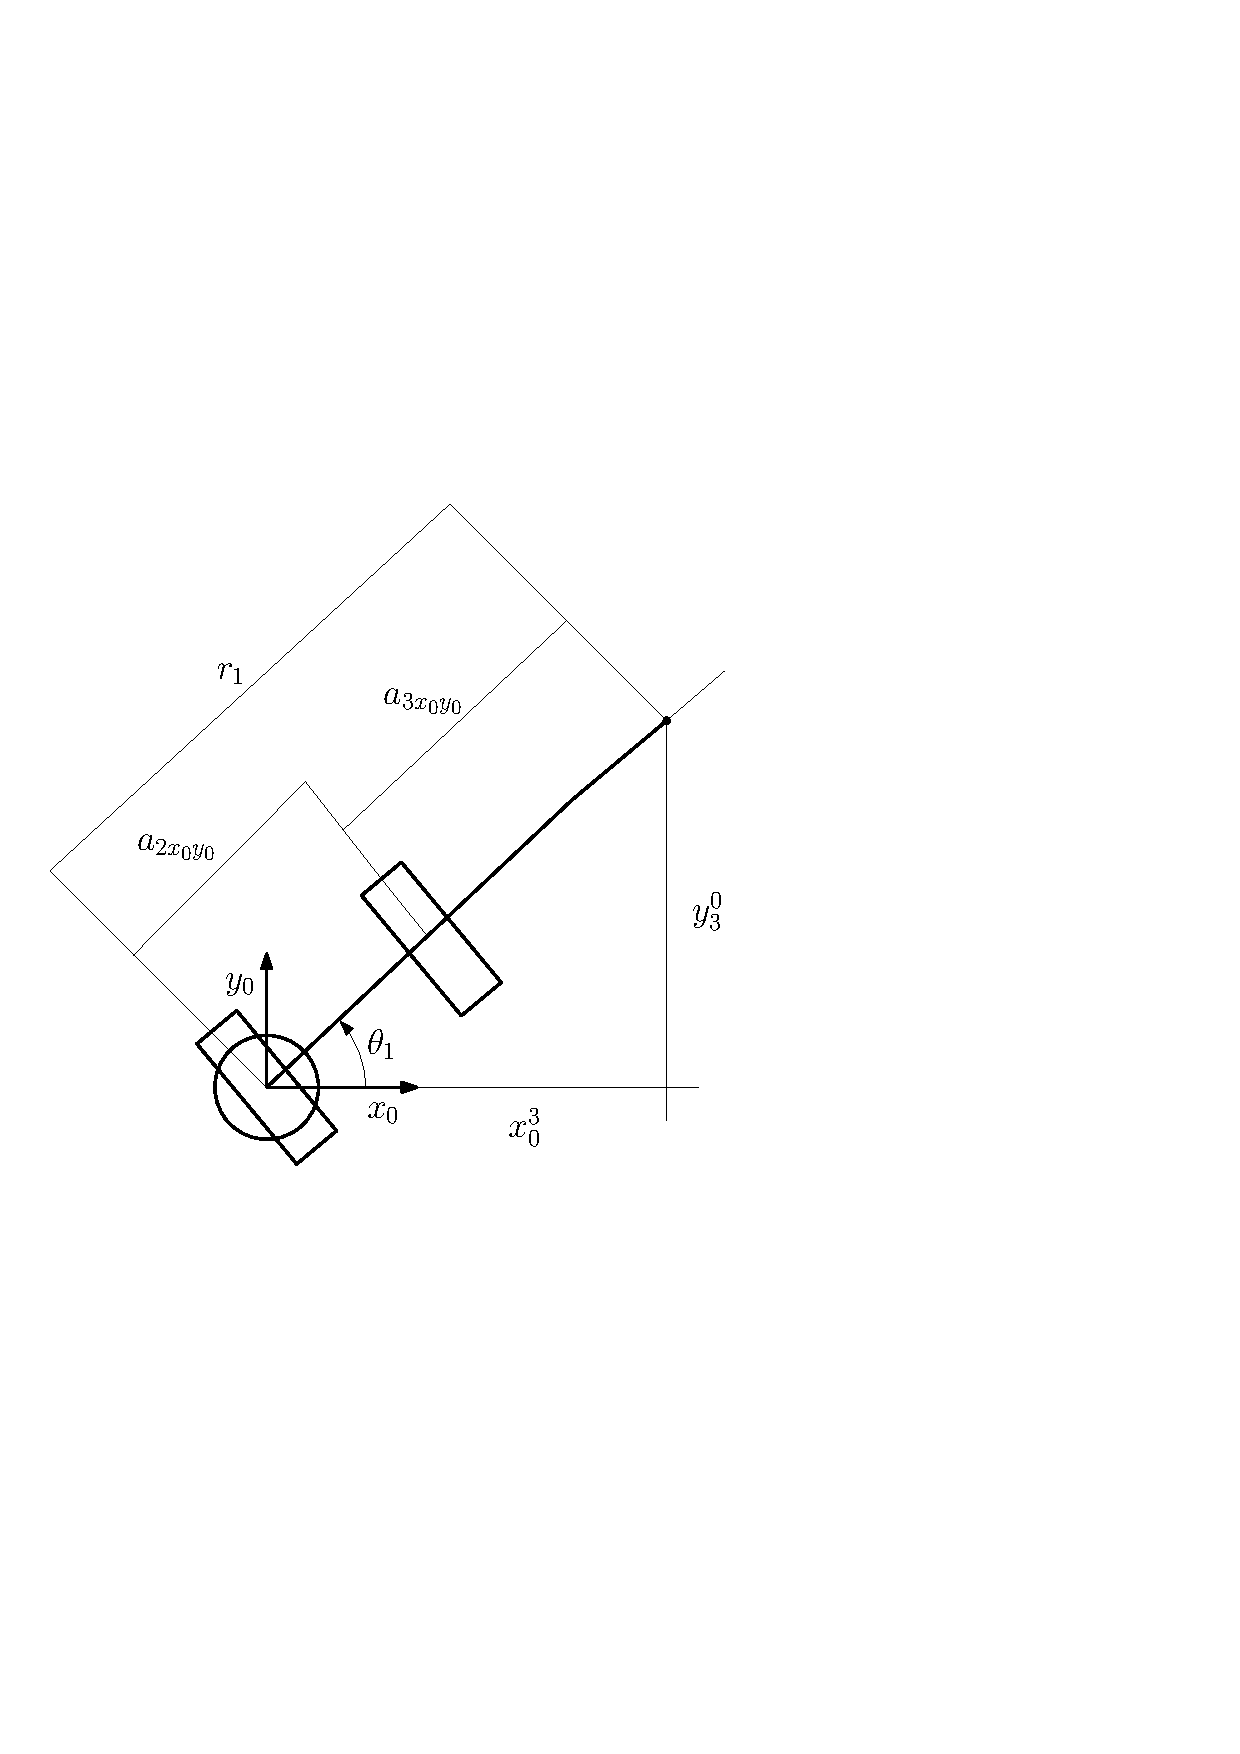
\includegraphics[width=0.5\textwidth]{2.pdf}\\
     Рисунок 2.3.2 Вид схемы сверху (проекция $x_0 y_0$).\\
\end{center}


Обозначим нулевую систему координат и угол вращения $\theta_1$ (можно было бы ещё обозначить известные параметры $a_2$ и  $a_3$, но в данной проекции отображаются $но в данном случае мы наблюдаем лишь их проекции. (мне кажется больше в скобках ничего не нужно)$не явные(известные) значения этих параметров, а их проекции на плоскость $x_0 y_0$, которые соответственно изменяются с изменениями угла, поэтому не указываются на таком виде). Можно заметить, что искомый угол $\theta_1$ выражается через отношение $y_3^0$ $x_3^0$ таким образом можно записать:$Можно заметить, что искомый угол можно выразить как$\\
$$\theta_1=arctg(\frac{y_3^0}{x_3^0});$$

\item[3.] Далее рассмотрим вид спереди данной системы, придав звеньям некоторое смещение $Не уверен, но мне кажется что комментарии не нужны$(для более наглядного выражения углов). Тут можно выделить неоднозначность решения ОЗК, поскольку можно заметить, что прийти в данную точку возможно несколькими вариантами смещения, к примеру:\\

\begin{center}
    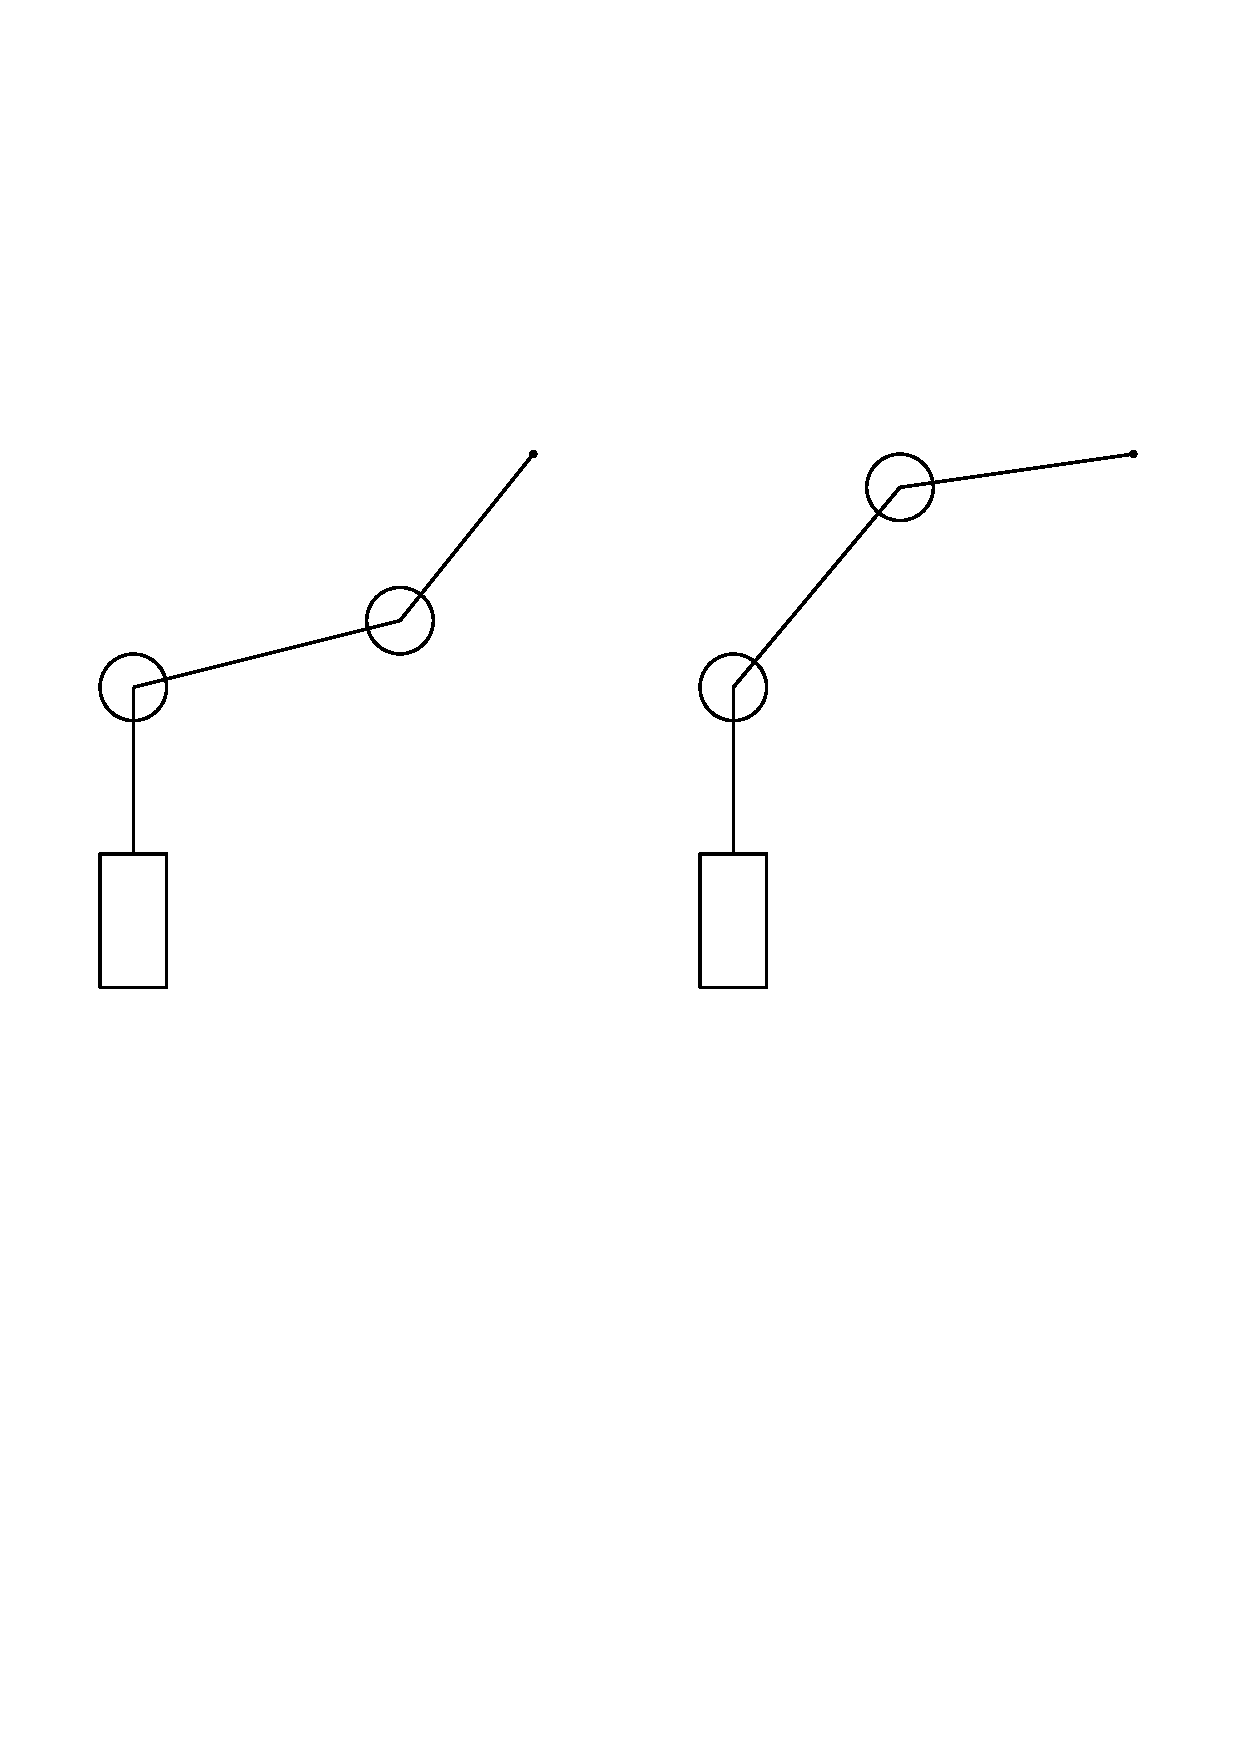
\includegraphics[width=0.55\textwidth]{1.pdf}\\
    а) Второе сочленение расположено снизу    б) Второе сочленение расположено сверху.\\
     Рисунок 2.3.3 схема манипулятора для некоторых одинаковых коэффициентов рабочего инструмента.\\
     $Рисунок 2.3.3 схема манипулятора для некоторых одинаковых коэффициентов рабочего инструмента.а) Второе сочленение расположено снизу, б) второе сочленение расположено сверху\\$%Вроде обычно так обозначают, либо в данном случае можно вообще без объяснения, если кратко то я могу ещё попридираться к этому
\end{center}
%Каждая конфигурация при решении ОЗК ограничивает рабочую облась, поэтому при решении задачи отдается предпочтение конфигурации которая в большей степени удовлетворяет достижению необходимой нам рабочей области.
Пусть будем рассматривать вариант с верхним расположением второго сочленения.\\%Для примера рассмотрим вариант ...
Итак, здесь помимо обозначения нулевой системы координат(можем обозначить только $z_1$, поскольку она является единственной не перпендикулярной осью вращения и задает своё изменение для $x_0$ и $y_0$) и углов вращения($\theta_2$ от оси,  $\theta_3$ от продолжения второго звена) можно обозначить параметры $d_1$, $a_2$ и $a_3$, поскольку их величины в данной проекции не изменяются. Также можно задать вспомогательные величины углов и длин: соединение первого и третьего сочленения $r_3$, достроение до треугольника $r_1$ и $r_2$, а также углы $\phi_1$, $\phi_2$, $\phi_3$.\\
%Мне кажется слишком много отступлений в скобочках, возможно я сейчас невыспавшийся злой и придираюсь, но я теряю мысль пока читаю отступления.

\begin{center}
    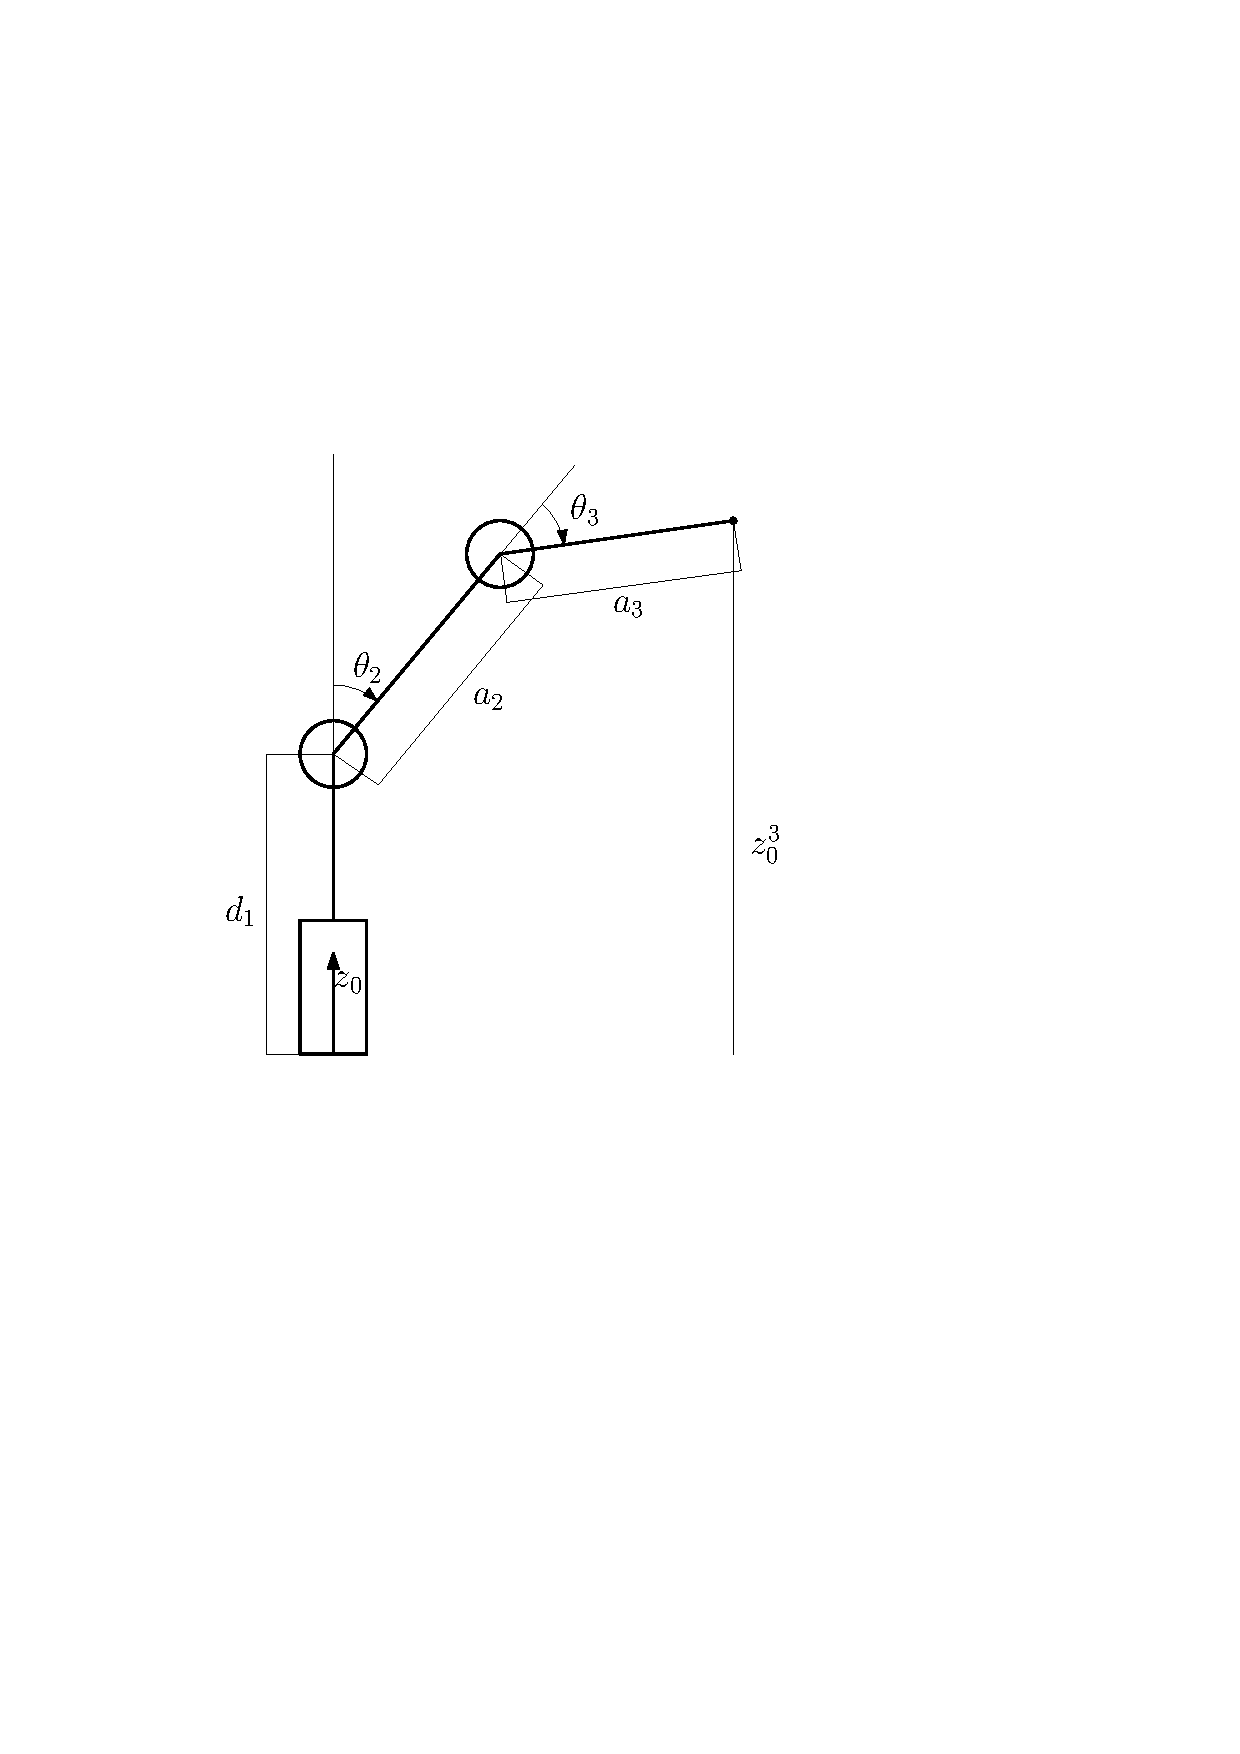
\includegraphics[width=0.4\textwidth]{3.pdf}\\
     Рисунок 2.3.4 Вид схемы спереди (проекция $x_0z_0$).\\
\end{center}

Рассмотрим поподробнее схему между вторым, третьим и инструментальным звеньями.\\

\begin{center}
    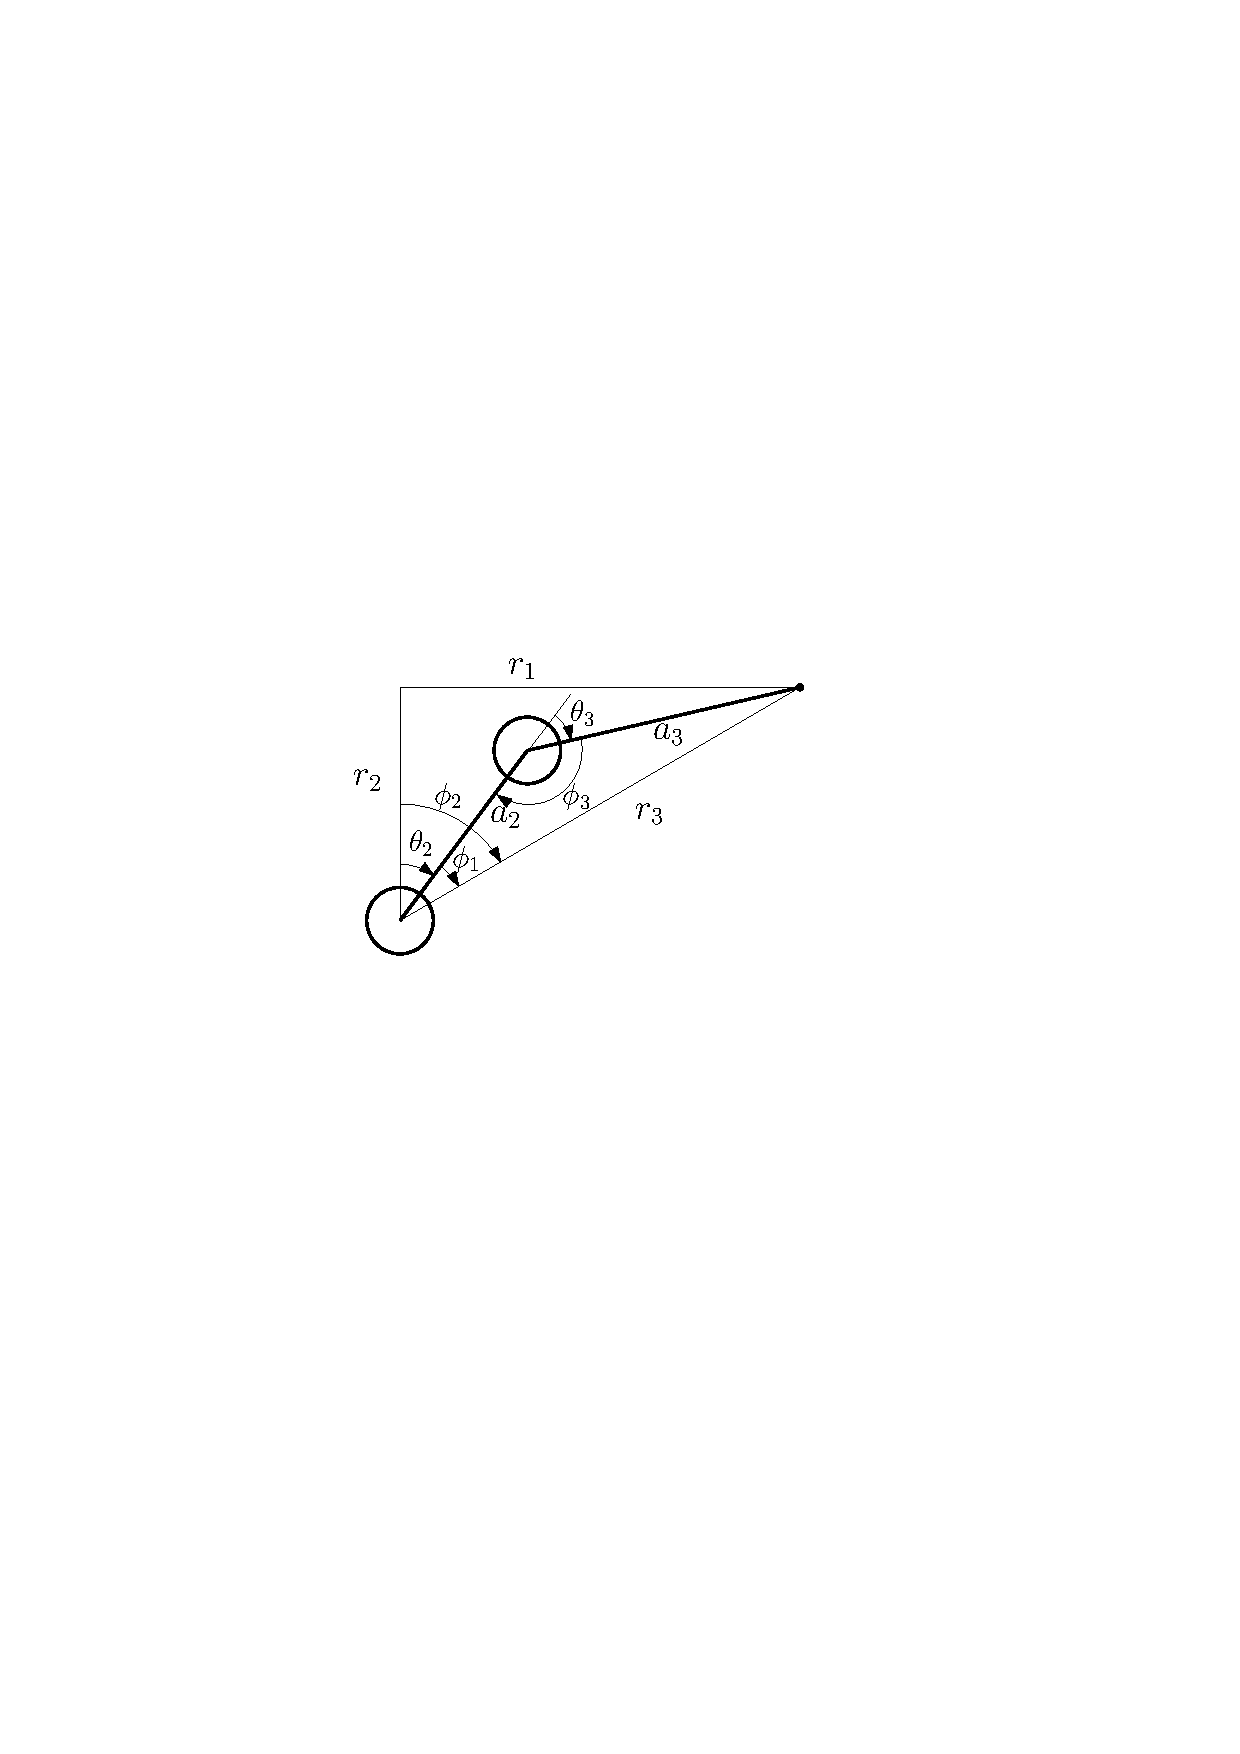
\includegraphics[width=0.5\textwidth]{4.pdf}\\
         Рисунок 2.3.5 Приближенное изображение схемы с необходимыми обозначениями. \\

\end{center}

Можно представить угол $\theta_2$ как разницу между углами $\phi_2$ и $\phi_1$:\\
$$\theta_2 = \phi_2 - \phi_1$$
- где $\phi_2$ видно из рисунка (треугольник, образованный сторонами $r_1$, $r_2$ и $r_3$ прямоугольный, $\phi_2$ определяет отношение катетов);
$$\phi_2 = arctg(\frac{r_1}{r_2})$$
- $r_2$ находится как разность между $z_0^3$ и $d_1$: \\
$$r_2=z_3^0 - d_1$$
- $r_1$ определяется из предыдущей проекции ($x_0y_0$) как сумма проекций $a_{2x0y0}$ $a_{3x0y0}$, которые в свою очередь определяются через теорему Пифагора:\\ $$r_1=a_{2x0y0}+a_{3x0y0}=\sqrt{(x_3^0)^2+(y_3^0)^2}$$
- $\phi_1$ находим через теорему косинусов в треугольнике, образованном сторонами $a_2$, $a_3$, $r_3$:\\
$$a_3^2 = a_2^2 + r_3^2 - 2 a_2 r_3 cos\phi_1$$
$$cos\phi_1 = \frac{a_2^2 + r_3^2 - a_3^2}{2 a_2 r_3} \rightarrow \phi_1 = arccos(\frac{a_2^2 + r_3^2 - a_3^2}{2 a_2 r_3})$$
- $r_3$ находится так же по теореме Пифагора:\\
%Вставить обозначения векторов
$$r_3=\sqrt{r_1^2+r_2^2}=\sqrt{(x_3^0)^2+(y_3^0)^2)+(z_3^0 - d_1)^2}$$
Таким образом получаем:\\
$$\theta_2=arctg(\frac{r_1}{r_2}) - arccos(\frac{a_2^2 + r_3^2 - a_3^2}{2 a_2 r_3})$$
$$ \theta_2=arctg(\frac{\sqrt{(x_3^0)^2+(y_3^0)^2}}{z_3^0-d_1}) - arccos(\frac{a_2^2 + ((x_3^0)^2+(y_3^0)^2)+(z_3^0 - d_1)^2) - a_3^2}{2 a_2 \sqrt{(x_3^0)^2+(y_3^0)^2)+(z_3^0 - d_1)^2}}) $$

Далее рассмотрим нахождение угла $\theta_3$, из рисунка 2.3.5 видно:
$$\theta_3=180-\phi_3$$
Далее через теорему косинусов в треугольнике ($a_2$, $a_3$, $r_3$) определяется угол $\phi_3$:\\
$$r_3^2=a_2^2+a_3^2 - 2cos\phi_3 a_2 r_3 \rightarrow \phi_3 = arccos(\frac{a_2^2 + a_3^2 -r_3^2}{2a_2 r_3})$$
$$\theta_3=180-arccos(\frac{a_2^2 + a_3^2 -r_3^2}{2a_2 r_3})=180-arccos(\frac{a_2^2 + a_3^2 -((x_3^0)^2+(y_3^0)^2)+(z_3^0 - d_1)^2)}{2a_2 \sqrt{(x_3^0)^2+(y_3^0)^2)+(z_3^0 - d_1)^2}})$$

 \end{enumerate}

\section{Практическое задание}

\paragraph*{3.1 Описание практической части\\}

\hspace*{\parindent}Практическая часть лабораторной работы состоит из нескольких задач:\\

\begin{enumerate} 
\item[1.] Прочитать и постараться понять предложенный теоретический материал, представленный выше.
\item[2.] Собрать робот-манипулятор из наборов \textit{LEGO}.
\item[3.] Измерить и рассчитать для него параметры Денавита - Хартенберга.
\item[4.] По полученным параметрам расписать ПЗК системы.
\item[5.] А также ОЗК системы.
\item[6.] Проверить правильность своих расчетов посредством подстановки прямой и обратной задач в пакете \textit{Scilab}.
\item[7.] Написать программу, позволяющею по входным параметрам (координатам в обобщенной системе) перемещать рабочий инструмент (хват) в заданное положение и определять свои параметры в текущий момент (углы вращения по входным координатам)
\item[8.] Написать программу, позволяющею по входным параметрам (углам вращения) перемещать рабочий инструмент (хват) в заданное положение и определять свои параметры в текущий момент (координаты обобщенной системы по входным углам вращения).
\item[9.] Также в пакете \textit{Scilab} построить траектории движения и сравнить с имеющийся на готовом роботе. 
 \end{enumerate}

\end{document}


